\section{Network Architectures}
\begin{frame}{}
    \LARGE Diffusion Models: \textbf{Network Architectures}
\end{frame}

\begin{frame}[allowframebreaks]{Network Architectures}
\begin{itemize}
    \item Diffusion models commonly use U-Net architectures with ResNet blocks and self-attention layers to represent $\epsilon_\theta(x_t, t)$.
    \item Time is encoded using sinusoidal positional embeddings or random Fourier features.
\end{itemize}
\begin{figure}
    \centering
    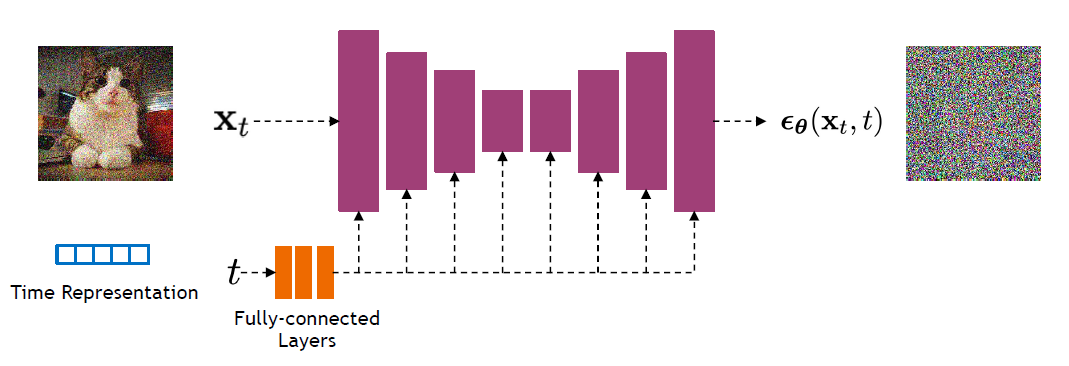
\includegraphics[height=0.7\textheight, width=\textwidth, keepaspectratio]{images/diffusion/diff_7.png}
\end{figure}

\framebreak
\begin{figure}
    \centering
    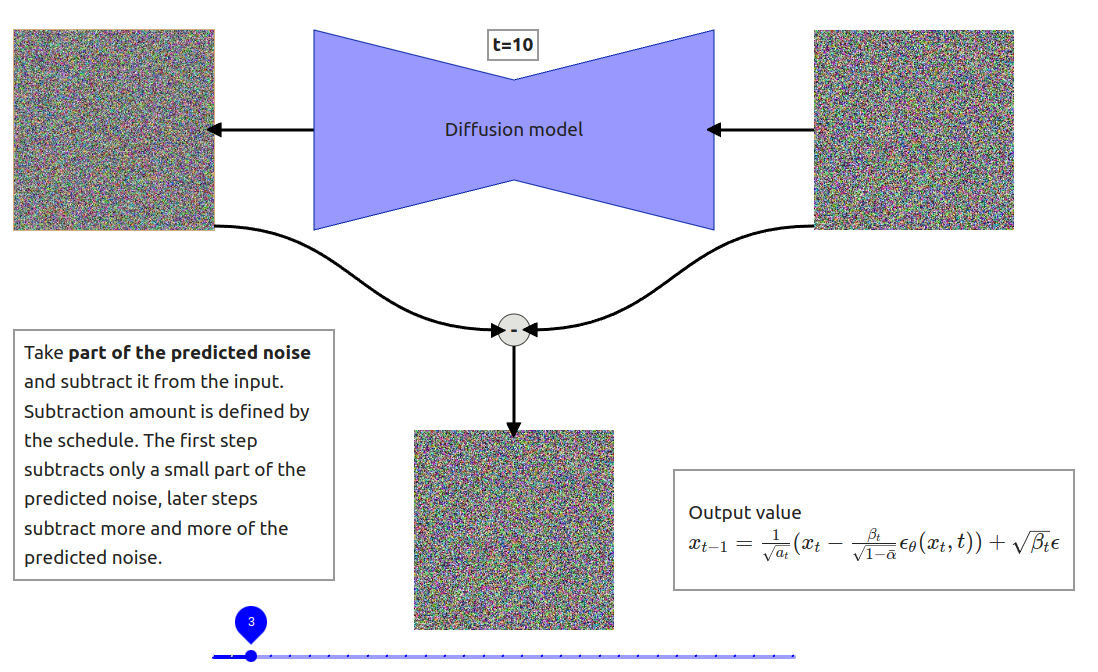
\includegraphics[height=0.9\textheight, width=\textwidth, keepaspectratio]{images/diffusion/architecture-network.png}
\end{figure}

\framebreak
\begin{figure}
    \centering
    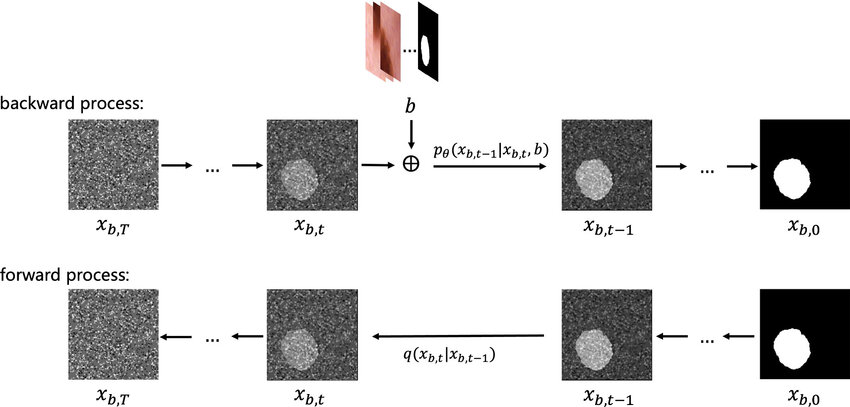
\includegraphics[height=0.9\textheight, width=\textwidth, keepaspectratio]{images/diffusion/architecture-forward-backward.png}
\end{figure}
\end{frame}

\begin{frame}{Connection to VAEs}
\begin{columns}
    \begin{column}{0.7\textwidth}
    \begin{itemize}
        \setlength{\itemsep}{0.75em}
        \item Diffusion models can be viewed as a special form of hierarchical VAEs (one VAE after another).
        \item In diffusion models:
        \begin{itemize}
            \setlength{\itemsep}{0.5em}
            \item The encoder is fixed.
            \item The latent variables have the same dimension as the data.
            \item The denoising model is shared across different timesteps.
            \item The model is trained with a reweighted variational bound.
        \end{itemize}
    \end{itemize}
    \end{column}

    \begin{column}{0.3\textwidth}
    \begin{figure}
        \centering
        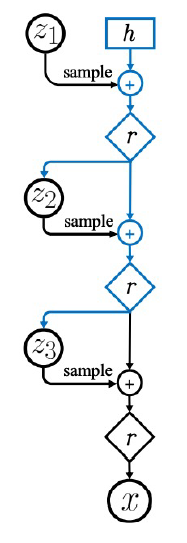
\includegraphics[height=0.8\textheight, width=\textwidth, keepaspectratio]{images/diffusion/diff_8.png}
    \end{figure}
    \end{column}
\end{columns}
\end{frame}
